\begin{enumerate}[label=\thesection.\arabic*.,ref=\thesection.\theenumi]
\numberwithin{equation}{enumi}

\item The Block diagram of a system is illustrated in the figure shown, where $X(s)$ is the input and $Y(s)$ is the output. Draw the equivalent signal flow graph.
\renewcommand{\thefigure}{\theenumi.\arabic{figure}}

\begin{figure}[!ht]
\centering
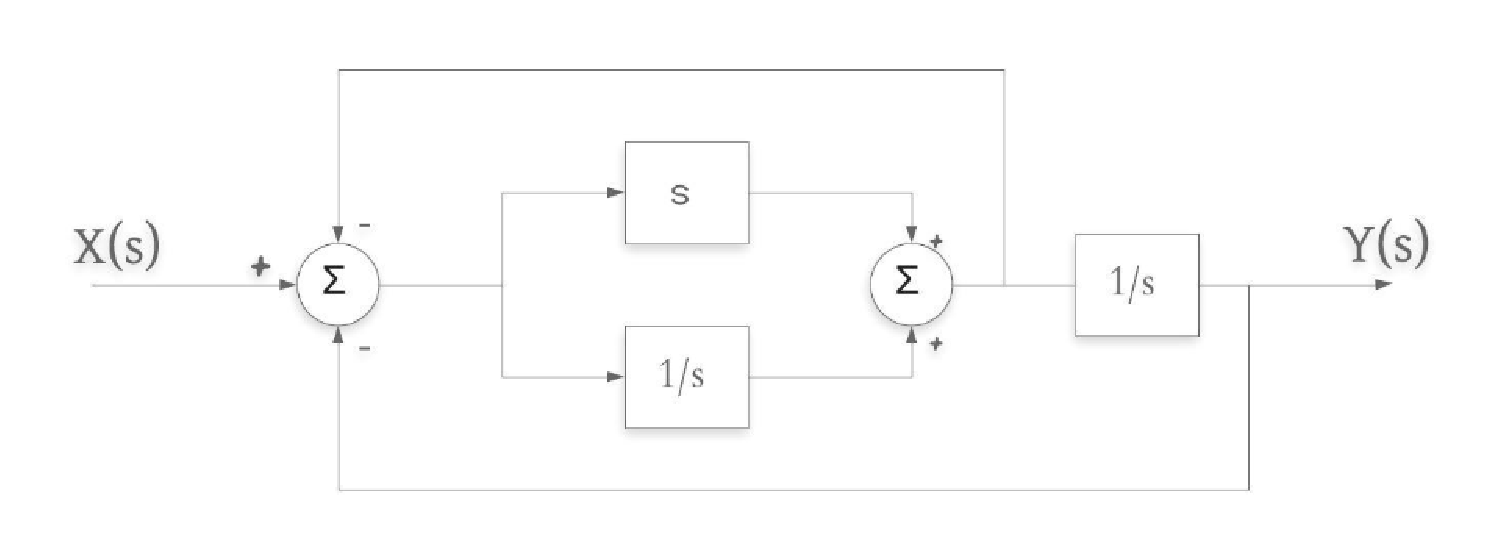
\includegraphics[width=\columnwidth]{./figs/ee18btech11003/pic1.eps}
\caption{}
\label{fig:sec_order}
\end{figure}
\solution
Signal flow graph of given above block diagram is
\begin{figure}[!ht]
\centering
\includegraphics[width=\columnwidth]{./figs/ee18btech11003/signal_flow.eps}
\caption{signal flow graph}
\label{fig:sec_order}
\end{figure}
%
\renewcommand{\thefigure}{\theenumi}
\item Draw all the forward paths and compute the respective gains.
\renewcommand{\thefigure}{\theenumi.\arabic{figure}}
\solution
Here, 
\begin{align}
P_1=\frac{s}{s}=1
\end{align}

\begin{figure}[!ht]
\centering
\includegraphics[width=\columnwidth]{./figs/ee18btech11003/P1.eps}
\caption{P1}
\label{fig:sec_order}
\end{figure}

 
\begin{align}
P_2=(1/s)(1/s)=1/s^2
\end{align}

\begin{figure}[!ht]
\centering
\includegraphics[width=\columnwidth]{./figs/ee18btech11003/P2.eps}
\caption{P2}
\label{fig:sec_order}
\end{figure}
\renewcommand{\thefigure}{\theenumi}

\item Draw the loops and calculate the respective gains.\renewcommand{\thefigure}{\theenumi.\arabic{figure}}
\\
\solution 
\begin{align}
L_1=(-1)(s)=-s
\end{align}

\begin{figure}[!ht]
\centering
\includegraphics[width=0.3\textwidth]{./figs/ee18btech11003/L1.eps}
\caption{L1}
\label{fig:sec_order}
\end{figure}


\begin{align}
L_2=\frac{s}{-s}=-1
\end{align}

\begin{figure}[!ht]
\centering
\includegraphics[width=0.3\textwidth]{./figs/ee18btech11003/L2.eps}
\caption{L2}
\label{fig:sec_order}
\end{figure}


\begin{align}
L_3=(\frac{1}{s})*(-1)=\frac{-1}{s}
\end{align}

\begin{figure}[!ht]
\centering
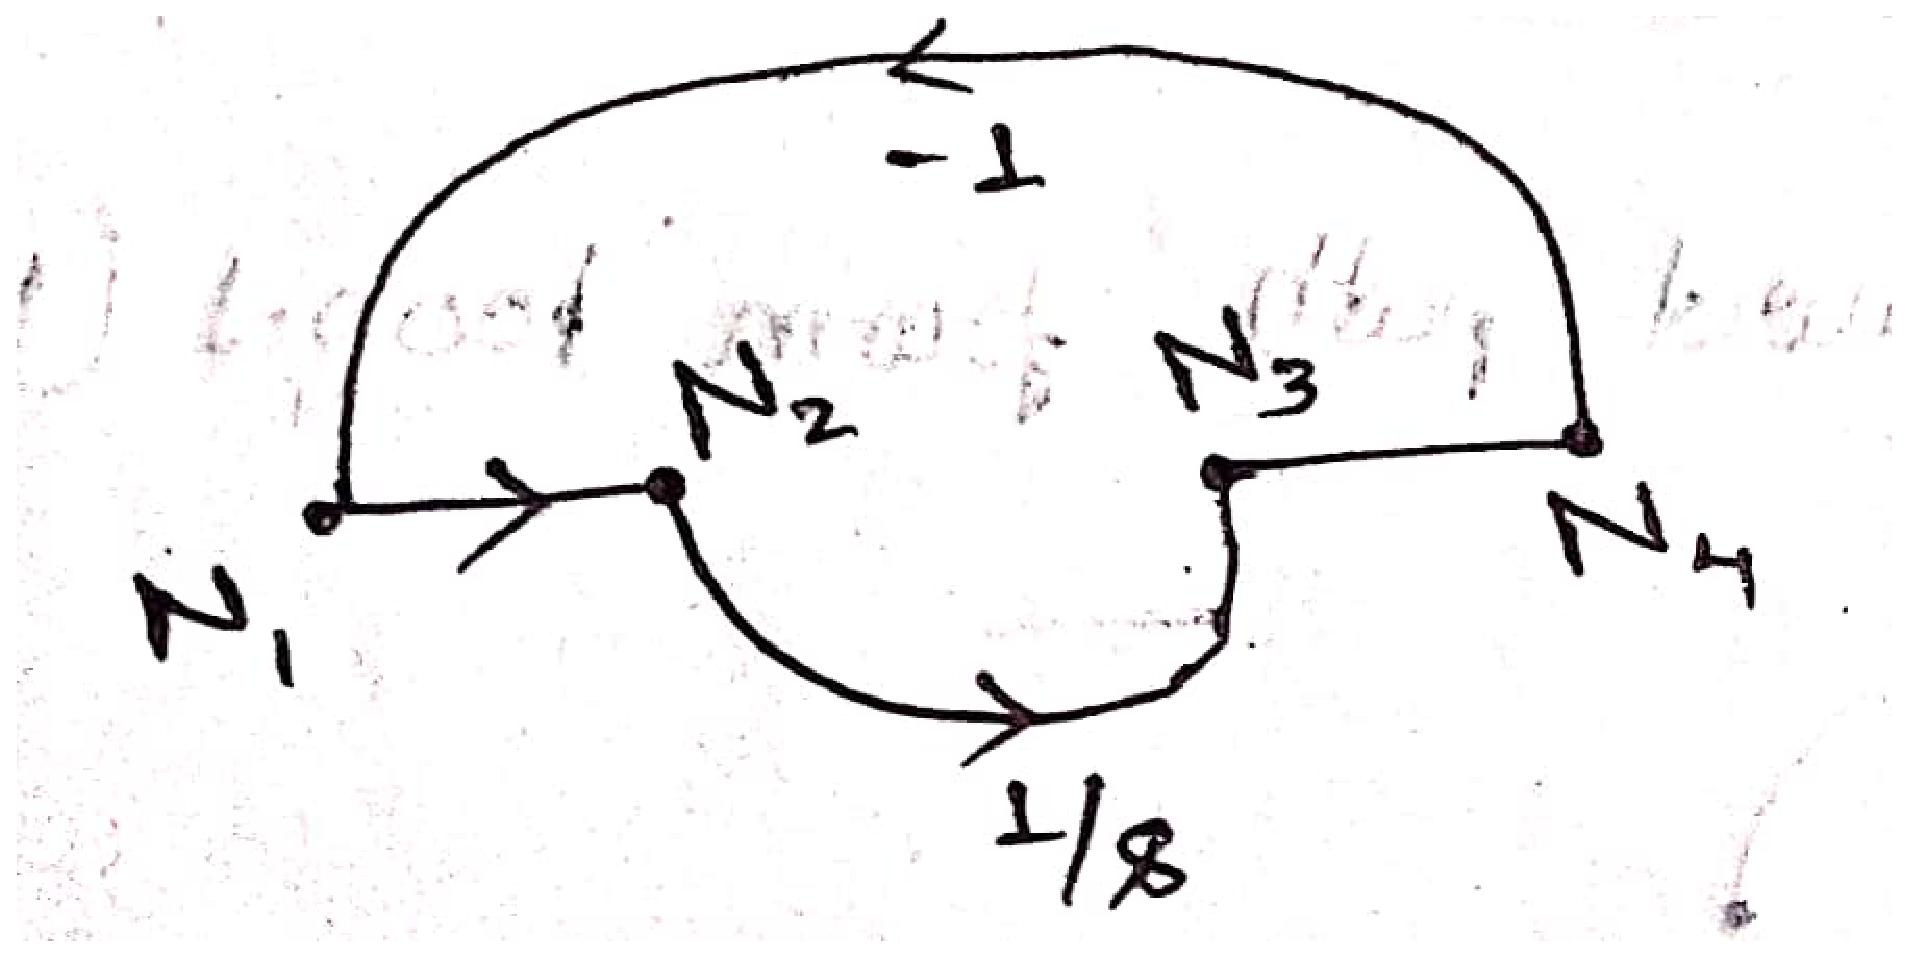
\includegraphics[width=0.3\textwidth]{./figs/ee18btech11003/L3.eps}
\caption{L3}
\label{fig:sec_order}
\end{figure}


\begin{align}
L_4=(\frac{1}{s})*(\frac{1}{s})8(-1)=\frac{-1}{s^2}
\end{align}

\begin{figure}[!ht]
\centering
\includegraphics[width=0.3\textwidth]{./figs/ee18btech11003/L4.eps}
\caption{L4}
\label{fig:sec_order}
\end{figure}
\renewcommand{\thefigure}{\theenumi}

\item State Mason's Gain formula and explain the parameters through a table.
\\
\solution 
According to Mason's Gain Formula,
\begin{align}
T = \frac{Y(s)}{X(s)} 
\end{align}
\begin{align}
T = \frac{\sum_{i=1}^{N} P_i\Delta_i}{\Delta}
\end{align}
\item  Find the transfer function using Mason's Gain Formula.
\renewcommand{\thefigure}{\theenumi.\arabic{figure}}
%
\\
\solution 
%\begin{align}
% H(s)=\frac{Y(s)}{X(s)} 
%\end{align}

%Options -
% \begin{align}
% (A) - H(s)=\frac{s^2+1}{s^3+s^2+s+1}
% \end{align}
% \begin{align}
% (B) - H(s)=\frac{s^2+1}{s^3+2s^2+s+1}
% \end{align}
% \begin{align}
% (C) - H(s)=\frac{s^2+1}{s^2+s+1}
% \end{align}
% \begin{align}
% (D) - H(s)=\frac{s^2+1}{2s^2+1}
% \end{align}



Now, 

Pi is the ith forward path.
%$\Delta = 1 - (Sum of all individual loop gains)+(sum of gain products of all possible two non-touching loops)-(sum of gain products of all possible three non-touching loops)+...$
%$\Delta_i is obtained from \Delta by removing the loops which are touching the i^{th} forward path.$


$\Delta = 1-(L_1 + L_2 + L_3 + L_4)$

\begin{align}
L_1=(-1)(s)=-s
\end{align}

\begin{figure}[!ht]
\centering
\includegraphics[width=0.3\textwidth]{./figs/ee18btech11003/L1.eps}
\caption{L1}
\label{fig:sec_order}
\end{figure}


\begin{align}
L_2=\frac{s}{-s}=-1
\end{align}

\begin{figure}[!ht]
\centering
\includegraphics[width=0.3\textwidth]{./figs/ee18btech11003/L2.eps}
\caption{L2}
\label{fig:sec_order}
\end{figure}


\begin{align}
L_3=(\frac{1}{s})*(-1)=\frac{-1}{s}
\end{align}

\begin{figure}[!ht]
\centering
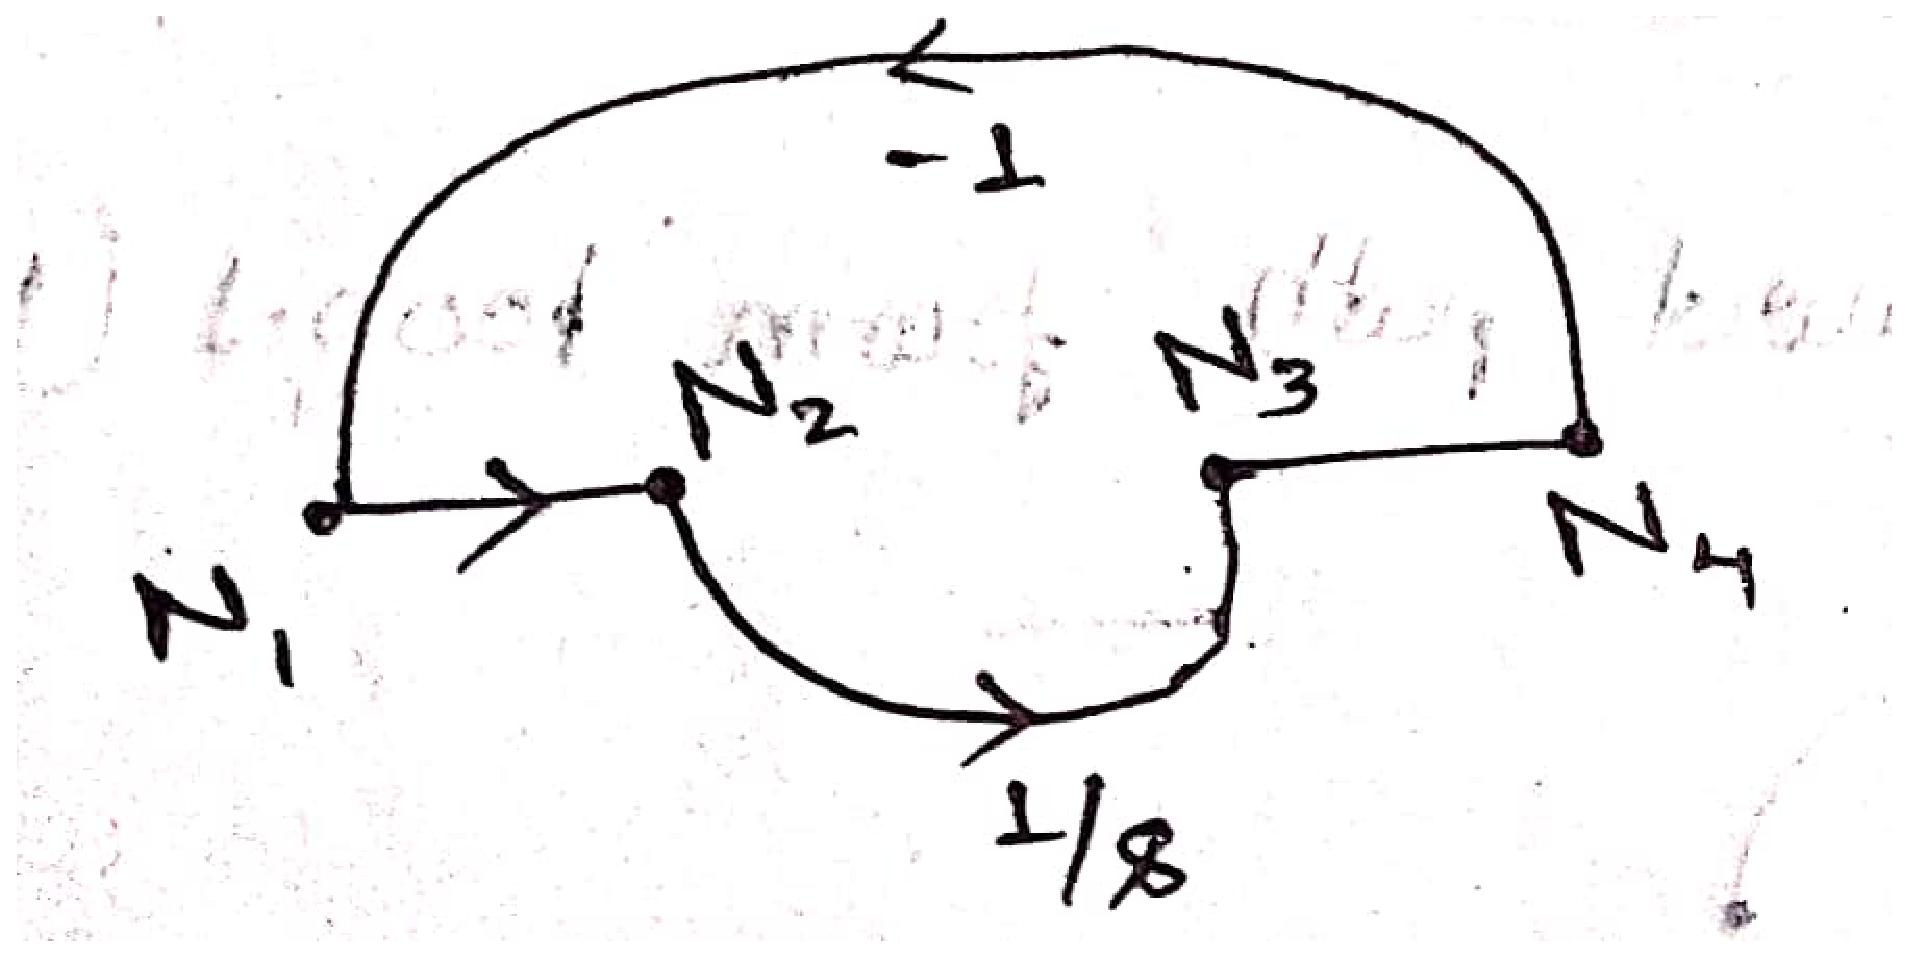
\includegraphics[width=0.3\textwidth]{./figs/ee18btech11003/L3.eps}
\caption{L3}
\label{fig:sec_order}
\end{figure}


\begin{align}
L_4=(\frac{1}{s})*(\frac{1}{s})8(-1)=\frac{-1}{s^2}
\end{align}

\begin{figure}[!ht]
\centering
\includegraphics[width=0.3\textwidth]{./figs/ee18btech11003/L4.eps}
\caption{L4}
\label{fig:sec_order}
\end{figure}


$\Delta = 1-(-s-1-\frac{1}{s}-\frac{1}{s^2})$
$\Delta = \frac{s^3+2s^2+s+1}{s^2}$

\begin{figure}[!ht]
\centering
\includegraphics[width=0.3\textwidth]{./figs/ee18btech11003/Delta1.eps}
\caption{Delta1}
\label{fig:sec_order}
\end{figure}


$\Delta_1 = 1$

\begin{figure}[!ht]
\centering
\includegraphics[width=0.3\textwidth]{./figs/ee18btech11003/Delta2.eps}
\caption{Delta2}
\label{fig:sec_order}
\end{figure}


$\Delta_2 = 1$

\begin{figure}[!ht]
\centering
\includegraphics[width=0.3\textwidth]{./figs/ee18btech11003/Delta3.eps}
\caption{Delta3}
\label{fig:sec_order}
\end{figure}


$\Delta_3 = 1$

\begin{figure}[!ht]
\centering
\includegraphics[width=0.3\textwidth]{./figs/ee18btech11003/Delta4.eps}
\caption{Delta4}
\label{fig:sec_order}
\end{figure}

$\Delta_4 = 1$

Here, 
\begin{align}
T=\frac{\sum_{i=1}^{N}(P_i)(\Delta_i)}{\Delta}
\end{align}

\begin{align}
T=\frac{P_1 \Delta_1+P_2 \Delta_2+P_3 \Delta_3+P_4 \Delta_4}{\Delta}
\end{align}

\begin{align}
T=\frac{1*1 +(\frac{1}{s^2})*1 + 0*1 + 0*1 }{\frac{s^3+2s^2+s+1}{s^2}}
\end{align}

\begin{align}
H(s)=\frac{s^2+1}{s^3+2s^2+s+1}
\end{align}
\renewcommand{\thefigure}{\theenumi}

\end{enumerate}
